% !TEX root = ../Thesis.tex
\myChapter[Radiation dose optimized expansion of the field of view]{Radiation dose optimized lateral expansion of the field of view in synchrotron radiation x-ray tomographic microscopy}\label{ch:Haberthuer2010}

David Haberthür\footremember{ana3}{Institute of Anatomy, University of Bern, Bern, Switzerland}\textsuperscript{,}\footnote{\href{mailto:haberthuer@ana.unibe.ch}{haberthuer@ana.unibe.ch}}\\
Christoph Hintermüller\footremember{psi3}{Swiss Light Source, Paul Scherrer Institut, Switzerland}\textsuperscript{,}\footremember{eth3}{Institute for Biomedical Engineering, University and ETH Zürich, Switzerland}\\
Federica Marone\footrecall{psi3}\\
Johannes C. Schittny\footrecall{ana3}\\
Marco Stampanoni\footrecall{psi3}\textsuperscript{,}\footrecall{eth3}\textsuperscript{,}\footnote{\href{mailto:marco.stampanoni@psi.ch}{marco.stampanoni@psi.ch}}\\\\
First published in: Journal of Synchrotron Radiation, 2010\\
\href{http://journals.iucr.org/s/}{Journal of Synchrotron Radiation}

\section{Abstract}
Volumetric data at micrometer level resolution can be acquired within a few minutes using synchrotron radiation based tomographic microscopy. The field of view along the rotation axis of the sample can easily be increased by stacking several tomograms, allowing  the investigation of long and thin objects at high resolution. On the contrary, an extension of the field of view in the perpendicular direction is non trivial. This paper presents an acquisition protocol which increases the field of view of the tomographic dataset perpendicular to its rotation axis. The acquisition protocol can be tuned as a function of the reconstruction quality and scanning time. Since the scanning time is proportional to the radiation dose imparted to the sample, this method can be used to increase the field of view of tomographic microscopy instruments while optimizing the radiation dose for radiation sensitive samples and keeping the quality of the tomographic dataset on the required level. This approach, dubbed wide field synchrotron radiation tomographic microscopy, can increase the lateral field of view up to five times. The method has been successfully applied for the three-dimensional imaging of entire rat lung acini with a diameter of \SI{4.1}{\milli\meter} at a voxel size of \SI{1.48}{\micro\meter}.

\section{Introduction}
The functional respiratory lung unit---the so-called acinus---is defined as the complex of alveolated airways distal of a last purely conducting airway, the terminal bronchiole~\cite{Rodriguez1987}. The total of all acini forms the lung parenchyma, the area where the pulmonary gas-exchange takes place. While the structural development of the gas-exchange region including the alveolar septa is quite well characterized~\cite{Schittny2007a,Schittny2008,Mund2008}, the development of the three-dimensional structure of its functional unit---of the acini---was not much studied due to the lack of suitable methods.

It is our goal to study the branching pattern of the acinar airways as well as the airflow within it. Tomographic methods, in particular synchrotron radiation based tomographic microscopy can access this kind of information nondestructively and noninvasively.

In order to visualize the thin sheets of tissue (alveolar septa) forming the gas-exchanging alveoli, a resolution in the order of one micron is required. An entire acinus is usually larger than the field of view of the tomographic microscope~\cite{Rodriguez1987,Weibel2009}, being the latest limited by the chosen optical configuration. Usually, a large field of view resulting in a large sample volume can only be acquired with low magnification and vice-versa. Lab-based micro-computed tomography stations (\micro CT) could potentially be used to study acini, but the resolution of such systems is too low to resolve all alveolar septa. Even if \micro CT stations are catching up, synchrotron radiation based tomographic microscopy beamlines provide the necessary high resolution combined with unmatched image quality.

Up to now, the price to pay for this high resolution was a limited field of view. For instance at the TOMCAT beamline \cite{Stampanoni2007} at the Swiss Light Source, Paul Scherrer Institute, Villigen, Switzerland, the field of view at a 10$\times$ magnification (\SI{0.74}{\micro\meter} voxel size) is limited to 1.52$\times$\SI{1.52}{\milli\meter}, insufficient for the imaging of an entire acini at high resolution.

Increasing the field of view perpendicular to the rotation axis of the sample cannot easily be achieved by placing tomographic datasets next to each other. It is instead necessary to merge several projections overlapping the desired field of view prior to tomographic reconstruction. Obviously, to satisfy the sampling theorem, increasing the field of view also requires to acquire more projections, finally resulting in an increased acquisition time.

We developed such a method to merge several independently acquired sets of projections to increase the field of view of the resulting tomographic dataset. In addition, by optimization of the number of recorded projections, we established different scanning protocols with a user-defined balance between acquisition time and image quality.

Because the total acquisition time is directly linked to the radiation imparted to the sample, it is obvious that such protocols also affect radiation damage and constitute an important optimization tool for radiation sensitive experiments.

\section{Materials and Methods}\label{sec:materials and methods}
\subsection{Sample Preparation}
Rat lung samples, prepared according to \citet{Tschanz2002} and \citet{Luyet2002} were used as test objects. Briefly, lungs of Sprague-Dawley rats were filled with \SI{2.5}{\percent} glutaraldehyde (\cf{CH2(CH2CHO)2}) in \SI{0.03}{\Molar} potassium-phosphate buffer (pH 7.4) by instillation via tracheotomy at a constant pressure of \SI{20}{\centi\meter} water column. In order to prevent recoiling of the lung, this pressure was maintained during glutaraldehyde-fixation for a minimum of two hours. Subsequently, the lungs were dissected free and immersed in toto in the same fixative at a temperature of \SI{4}{\celsius} for at least \SI{24}{\hour}.

The samples were postfixed with \SI{1}{\percent} osmium tetroxide (\cf{OsO4}) and stained with \SI{4}{\percent} uranyl nitrate (\cf{UO2(NO3)2}) to increase the x-ray absorption contrast, dehydrated in a graded series of ethanol and embedded in paraffin using Histoclear (Merck KGaA, Darmstadt, Germany) as an intermedium. The lung samples were mounted onto standard scanning electron microscopy sample holders (PLANO GmbH, Wetzlar, Germany) using paraffin~\cite{Tsuda2008}.

The handling of animals before and during the experiments, as well as the experiments themselves, were approved and supervised by the Swiss Agency for the Environment, Forests and Landscape and the Veterinary Service of the Canton of Bern, Switzerland.

\subsection{Synchrotron radiation tomographic microscopy}
The experiments were performed at the TOMCAT beamline at the Swiss Light Source, Paul Scherrer Institut, Villigen, Switzerland. The samples were scanned at \SI{12.6}{\kilo\electronvolt}. After penetration through the sample, the x-rays were converted into visible light by a YAG:Ce scintillator (\SI{18}{\micro\meter} thickness, Crismatec Saint-Gobain, Nemours, France). Projections were magnified by diffraction limited microscope optics (10$\times$ magnification) and digitized by a high-resolution 2048$\times$2048 pixel CCD camera (pco.2000, PCO AG, Kelheim, Germany) with 14 bit dynamic range. The detector was operated in 2$\times$2 binning mode. As a result, the pixel size was \SI{1.48}{\micro\meter} and the exposure time was \SI{175}{\milli\second}.

Projections $I_{Pr}$ were recorded at equiangular positions between \SI{0}{\degree} and \SI{180}{\degree}. The exact number of angular projections depended on the selected scan protocol, as described in section~\ref{subsec:increasing the field of view}. Additionally, for each protocol a set of dark ($I_{D}$) and flat images ($I_{F}$) were recorded for noise and baseline correction, respectively. Further details of the imaging and reconstruction workflow at the TOMCAT beamline can be found in~\cite{Hintermueller2010}.

\subsection{Increasing the field of view}\label{subsec:increasing the field of view}
For parallel beam geometry, tomographic images are obtained at equidistant angles over a sample rotation of \SI{180}{\degree} as shown in Figure~\ref{fig:scanning-possibilities}(a). After reconstruction, the width of the image corresponds to the field of view of the camera.

Samples twice as large as the field of view can be imaged using scanning protocols based on a \SI{360}{\degree} off center sample rotation as shown in Figure~\ref{fig:scanning-possibilities}(b). Images recorded between \SI{180}{\degree} and \SI{360}{\degree} have to be flipped after acquisition: the projections obtained at angular position $\theta$ and $\theta$+\SI{180}{\degree} ($I_{Pr_{\theta}}$ and $I_{Pr_{\theta+\SI{180}{\degree}}}$) have to be stitched to one projection. The resulting images cover twice the field of view of the camera.

\begin{figure}
	\centering
	\caption{Covering the field of view of differently sized samples with one \SI{180}{\degree} scan (a), one \SI{360}{\degree} scan (b) or---in the case of the so called wide field scanning---with multiple subscans (three subscans, c). The filled segments mark the region of the sample that is covered while scanning the respective positions (Position 1: magenta/checkerboard, Position 2: yellow, Position 3: cyan/striped).}
	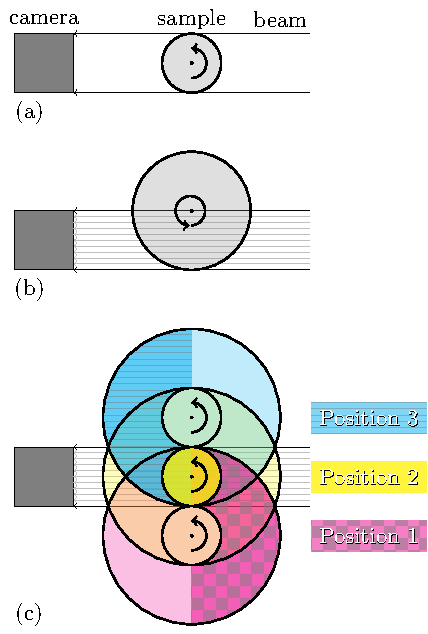
\includegraphics{img/Haberthuer2010/Fig01-FOV}
	\label{fig:scanning-possibilities}
\end{figure}

For tomographic scans covering a size wider than two fields of view, three or more \SI{180}{\degree}-scans taken at slightly overlapping positions are combined, as shown in Figure~\ref{fig:scanning-possibilities}(c). The projections of each subscan overlap slightly to facilitate the stitching of multiple projections into a single one. The cutline, i.\,e. the position where the merging takes place, is automatically determined according to a mean squared difference method~\cite{Hintermueller2010}.

A straightforward acquisition scheme would record an equal amount of projections for each of the individual subscans. As a consequence, to fulfill the sampling theorem in the lateral parts of the sample, oversampling the central parts of the sample would be necessary.

Since the total acquisition time per sample linearly scales with the total amount of recorded projections such an acquisition scheme obviously increases the total amount of beamtime for one sample without relevantly increasing the quality of the reconstructed tomographic data. Hence, such an oversampling is generally avoided.

Our goal was to find a good compromise between scanning time and image quality. We therefore devised an acquisition scheme for covering a wide field of view based on the assumption that a sufficient resolution and contrast can be achieved in the tomographic dataset, if the sampling theorem is individually fulfilled for each of the subscans. This results in a set of $i$ subscans with $P_{i}$ projections each. A simple example with $P_{2}=4$ and $P_{1}=P_{3}=8$ is shown in Figure~\ref{fig:projections}(a). Since each subscan $i$ has a different number of projections $P_{i}$, the stitching algorithm has to interpolate missing projections from adjacent projections (represented by the dotted lines in Figure~\ref{fig:projections}(b)) to generate a complete set of merged projections for reconstruction.

As a by-product, such an optimization of the individual number of projections $P_{i}$ for each subscan $i$ decreases the total acquisition time for one sample and thus the imparted radiation dose.

\begin{figure}
	\centering
	\caption{Wide field scan setup with three \SI{180}{\degree} scans; one central (yellow) and two lateral scans (magenta and cyan or top and bottom, respectively). In this drawing, four projections for the central and eight projections for each of the lateral scans have been recorded. The colors of the three positions correspond to the colors shown in Figure~\ref{fig:scanning-possibilities}(c). %
	(a): scanned projections %
	(b): scanned projections and additional interpolated projections (dotted) required to merge all projections.}
	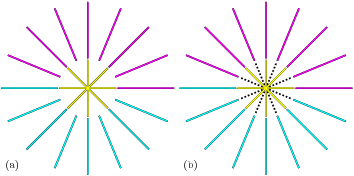
\includegraphics{img/Haberthuer2010/Fig02-Interpolation}
	\label{fig:projections}
\end{figure}	

We defined a gold standard protocol and several additional scanning protocols in order to compare different acquisition schemes. The gold standard protocol covers the desired field of view while fulfilling the sampling theorem---which states that for a detector width of $D$ pixels, we need to acquire a number of projections $P=D\frac{\pi}{2}$~\cite{Kak2002}---in all its regions, as shown in Figure~\ref{fig:SubScan-Setup}(a). In this case we need to achieve a field of view of 3072 pixels. The dark gray circle is the field of view that could be covered using a large detector with a size of 3072 pixels and recording $P=3072\frac{\pi}{2}=4825$ projections.

Using a detector with a size of 1024 pixels, this desired field of view could be covered with nine independent local tomography scans. Such an approach would require nine independent reconstructions and stitching of those nine reconstructed tomographic datasets into one dataset covering the full field of view. This method would also introduce artifacts at the edges of each of the nine sub-datasets which would lie inside the sample to be imaged.

While the chosen field of view of 3072$\times$3072 pixels can be covered using a detector of the size of 3072 pixels in one scan, we can cover the desired field of view with a much smaller detector, using a scanning protocol with three subscans from which we obtain merged projections. Figure~\ref{fig:SubScan-Setup}(b) shows how the desired field of view of 3072 pixels can be covered with a wide field scan, composed of one central and two half ring-scans, recorded with a small detector with a size of 1024 pixels and 4825 projections per subscan (a total of 14475 projections) which are then subsequently merged to 4825 large projections spanning the whole field of view. A further increase in the field of view can be obtained by simple iteration. Figures~\ref{fig:SubScan-Setup}(c)--(f) show such a setup for a five- or seven-fold increase.

\begin{figure}
	\centering
	\caption{Setup for different field of views. %
		(a): Desired field of view of 3072 pixel diameter. %
		(b): Wide field scanning protocol for covering the desired field of view of panel (a) with merged projections from one central and two half ring scans ($r_{1}$ and $r_{2}$). %
		(c): Desired field of view of 5120 pixel diameter. %
		(d): Wide field scanning protocol for covering the desired field of view of panel (c) with merged projections from one central and four half ring scans ($r_{1}$--$r_{4}$). %
		(e): Desired field of view of 7168 pixel diameter. %
		(f): Wide field scanning protocol for covering the desired field of view of panel (e) with merged projections from one central and six half ring scans ($r_{1}$--$r_{6}$).}%
	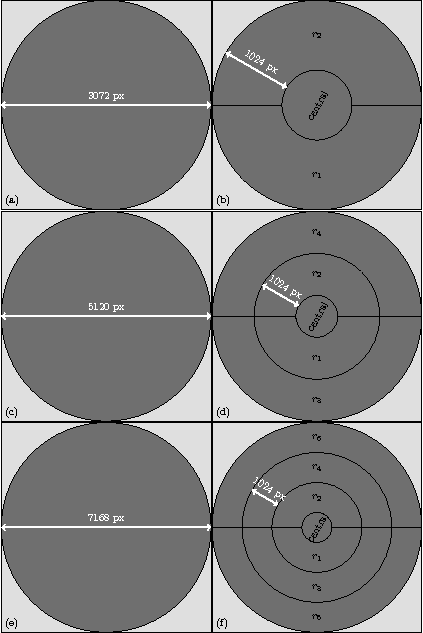
\includegraphics[width=.8\linewidth]{img/Haberthuer2010/Fig03-3-5-7}
	\label{fig:SubScan-Setup}
\end{figure}

\subsection{Quality guided protocols}\label{sec:quality guided protocols}
Taking the experimental constraints like desired field of view, available detector size, magnification and binning into account, a MATLAB-script calculates a set of acquisition protocols. Each such protocol contains the number of projections for each subscan linearly scaled in total amount of projections from a gold standard scan down to a protocol where the sampling theorem is far from being satisfied (Table~\ref{tab:protocols}). Through optimization of the number of recorded projections, a reduction of the total acquisition time by \SI{84}{\percent} (compared to the gold standard) was achieved.

Using a Shepp-Logan phantom~\cite{Shepp1974} with added Gaussian noise as a reference image, a simulated tomographic scan and subsequent reconstruction was calculated for each of these acquisition protocols. For each protocol we calculated the expected reconstruction quality using the difference image between the reconstruction of this protocol and the initial reference image. This simulated reconstruction quality was plotted against the total acquisition time (red dots in Figure~\ref{fig:NormalizedErrorPlot}).

The end-user---balancing between acquisition time and desired image quality---chooses one protocol from the presented set for scanning his sample. A file containing all the details of the chosen scan is written to disk, and parsed by a custom Python-script. This script interacts with the hardware control system at the TOMCAT beamline enabling an automated, unattended batch acquisition of all necessary subscans.

To assess the simulations in a real world example, we selected nineteen different acquisition protocols with varying number of projections to scan one single sample (details are specified in Table~\ref{tab:protocols}, including the calculated Quality for each protocol).

A scan covering the chosen field of view with nine independent local tomography scans, each with a field of view of 1024$\times$1024 pixels, would need a total of $P=9(1024\frac{\pi}{2})=14476$ projections. This protocol was not considered for this study, since the sampling theorem can be equally satisfied by acquiring the required amount of projections with one central and two ring scans, as defined in section~\ref{subsec:increasing the field of view}. Including an overlap of 100 pixels between the central and the ring scan, an equivalent wide field scanning protocol (Protocol A in Table~\ref{tab:protocols}) requires the acquisition of 13534 projections ($P_{A}=3(3072-200)\frac{\pi}{2}$).

Protocols B--T have been linearly scaled down with a decreasing number of acquired projections of the ring scans. To simplify interpolation and merging of the projections from each subscan, we only selected acquisition schemes where the number of projections of the inner and the outer subscans is the same or a multiple of two (see figure~\ref{fig:projections}). This constraint also led to a slight oversampling for protocol B, otherwise the number of projections for each subscan of this protocol ($5244=3\cdot874$) would not have scaled down nicely to the 874 projections used for protocol T.

All parameters of each protocol and each subscan (sample-position in relation to the beam, rotation angles and number of projections) were set in a preference-file, generated using aforementioned MATLAB-script. One rat lung sample was scanned using each of the 19 different protocols (B--T), without manual intervention, permitting a direct comparison of the reconstructed datasets.

\begin{table}
	\caption{Details of the 19 scanned protocols for this study (B--T): An unoptimized scan to cover the desired field of view of 3072 pixels with nine independent scans (with a detector width of 1024 pixels) would require to record a total of $P_{\textrm{Gold standard}}=9(1024)\frac{\pi}{2}=14476$ projections. The wide field scanning protocol (A) equivalent to this field of view only uses three subscans, resulting in a total number of projections of $P_{A} = 3(3072-200)\frac{\pi}{2}= 13534$. Three-dimensional reconstructions of the datasets marked with a light gray background are shown in Figure~\ref{fig:BvsT}.}
	\label{tab:protocols}
	\begin{tabular}{ccccccc}
		\toprule
		\multirow{2}{*}{Protocol} & \multicolumn{3}{c}{Projections for Subscan} & Total Number & Time/Radiation & Simulated\\
			& $\textrm{s}_{1}$ & $\textrm{s}_{2}$ & $\textrm{s}_{3}$        & of Projections & Dose [\%] & Quality [\%]\\
		\midrule
		A\footnote{Wide field scan equivalent to an unoptimized scan covering the field of view with nine independent scans.} & & & & 13534 & 100 & \\
		\rowcolor{lightgray} B\footnote{Gold Standard for this study} & 5244 & 5244 & 5244 & 15732 & 116 & 100\\
		C & 5244 & 2622 & 5244 & 13110 &  97 & 89\\
		D & 4370 & 4370 & 4370 & 13110 &  97 & 85\\
		E & 4370 & 2185 & 4370 & 10925 &  81 & 87\\
		F & 3934 & 3934 & 3934 & 11802 &  87 & 80\\
		G & 3934 & 1967 & 3934 & 9835  &  73 & 84\\
		H & 3496 & 3496 & 3496 & 10488 &  77 & 78\\
		I & 3496 & 1748 & 3496 & 8740  &  65 & 80\\
		J & 3060 & 3060 & 3060 & 9180  &  68 & 76\\
		K & 3060 & 1530 & 3060 & 7650  &  57 & 75\\
		\rowcolor{lightgray} L  & 2622 & 2622 & 2622 & 7866  &  58 & 72\\
		M & 2622 & 1311 & 2622 & 6555  &  48 & 69\\
		N & 2186 & 2186 & 2186 & 6558  &  48 & 67\\
		O & 2185 & 1093 & 2185 & 5463  &  40 & 62\\
		P & 1748 & 1748 & 1748 & 5244  &  39 & 61\\
		Q & 1748 & 874  & 1748 & 4370  &  32 & 55\\
		R & 1312 & 1312 & 1312 & 3936  &  29 & 46\\
		S & 874  & 874  & 874  & 2622  &  19 & 21\\
		\rowcolor{lightgray} T & 874  & 437  & 874  & 2185  &  16  & 20\\
		\bottomrule
	\end{tabular}
\end{table}

\subsection{Projection merging and tomographic reconstruction}
After acquisition of the three subscans per protocol, custom MATLAB functions read the parameters of the single subscans (e.\,g. sample name, amount of subscans, amount of dark and flat images) as well as the desired output-name and -suffix, and performed all necessary calculations, including: loading of the correct projections from each subscan; normalizing; interpolation; cutline detection; correct stitching of the images into wide field projections, and writing these merged projections as well as log files needed for the reconstruction to disk.

The merged projections were subsequently rearranged into sinograms, where the $n$\textsuperscript{th} sinogram is composed of the $n$\textsuperscript{th} line of every corrected projection. The $n$\textsuperscript{th} slice of the tomographic scan was reconstructed from the $n$\textsuperscript{th} sinogram using an FFT-based regridding algorithm~\cite{Dowd1999,Marone2008}. The 19 tomographic datasets were reconstructed on a computing cluster composed of five \SI{64}{\bit} Opteron machines with four cores and \SI{8}{\giga\byte} RAM each. The reconstructions resulted in an image stack covering a large sample volume of 2792$\times$2792$\times$1024 pixels, a nine-fold increase from the standard volume of 1024$\times$1024$\times$1024 pixels for one conventional scan.

\section{Results}\label{sec:Results}
\subsection{Image Merging and Reconstruction}\label{sec:Image Merging and Reconstruction}
Figure~\ref{fig:wide-field-scan-results}(a) shows corrected projections from three overlapping subscans prior to merging, including regions where the subscans are overlapping. Figure~\ref{fig:wide-field-scan-results}(b) shows one merged projection prior to reconstruction and Figure~\ref{fig:wide-field-scan-results}(c) shows one slice of the reconstructed dataset. The example shown in Figure~\ref{fig:wide-field-scan-results} was obtained using the highest number of projections and is therefore protocol B. One reconstructed slice covers a field of view of 2792$\times$2792 pixels (4.13$\times$\SI{4.13}{\milli\meter}), which is almost three times the size of what can be achieved with one single binned scan (1024 pixels or \SI{1.52}{\milli\meter}). %1024 * 1.48 um/px = 1.51552mm
The dashed circles on the reconstructed slice mark the start and the end of the overlap region.

\begin{figure}
	\centering
	\caption{Workflow of a wide field scan. The images show a rat lung sample from a Sprague-Dawley rat, obtained 21 days after birth, scanned with the acquisition protocol B (Table~\ref{tab:protocols}). %
			(a): Three corrected and independently acquired projections from subscans $s_1$--$s_3$ are shown. Each one is 1024\(\times\)1024 pixels large and covers a field of view of \SI{1.52}{\milli\meter}. Subscans $s_1$ and $s_2$ overlap by 141 pixels (red and green overlay), subscans $s_2$ and $s_3$ overlap by 138 pixels (blue and yellow overlay). %
			(b): Merged projection obtained from the three subscans shown in subfigure (a). Each merged projection has a size of 2792\(\times\)1024 pixels. Due to the overlap required to merge the projections, the width of the merged projections is slightly smaller than three times the width of the subscans. %
			(c): Cropped slice of the reconstructed tomographic dataset. The dashed red circles mark the start and end of the overlap region.}
	%%%%%%%%%%%%%%%%%%%%%%%%%%%%%%%%%%%
	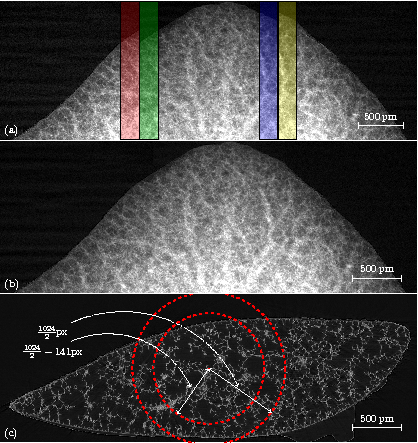
\includegraphics[width=\linewidth]{img/Haberthuer2010/Fig04-Workflow}
	\label{fig:wide-field-scan-results}
\end{figure}

Figure~\ref{fig:s2-wfs} shows the advantages of the wide field acquisition scheme. With---in this particular case---an enlargement of the field of view by almost a factor of three, it is possible to visualize entire acini at high resolution. For a conventional scan (fig.~\ref{fig:s2-wfs}(a)), the airway segments in the sample are only partially contained inside the dataset (magenta and yellow). The semitransparent airway segments are contained in the sample, but are not visible in the field of view of a dataset obtained with a conventional scan. Increasing the field of view (fig.~\ref{fig:s2-wfs}(b)) allows the visualization of those segments to their full extent. A third acinus (cyan) which was not visible in Figure~\ref{fig:s2-wfs}(a) can now easily be visualized.

\begin{figure}
	\centering
	\caption{Three-dimensional visualization of the distal-medial tip of the right lower rat lung lobe. The gray structure in the background shows a semitransparent view of the tomographic dataset with segmented airways. The foreground shows isosurfaces of terminal airways. The wireframe cube has a side length of 1024 pixels and encloses the field of view of one conventional scan. %
	(a): Conventional scan; the extracted airway segments (magenta and yellow or left and right, respectively) are only partially contained inside the total sample volume. Airway segments not contained in the dataset, but present in the sample are shown semitransparent. This conventional scan corresponds to a reconstruction of the central of the three wide field scan subscans. %
	(b): Wide field scan with increased field of view; the magenta (center) and yellow segment (right) show entire acini inside the dataset, the cyan segment (left) contains a partially cut acinus. All airway segments inside the sample are contained in the tomographic dataset.}
	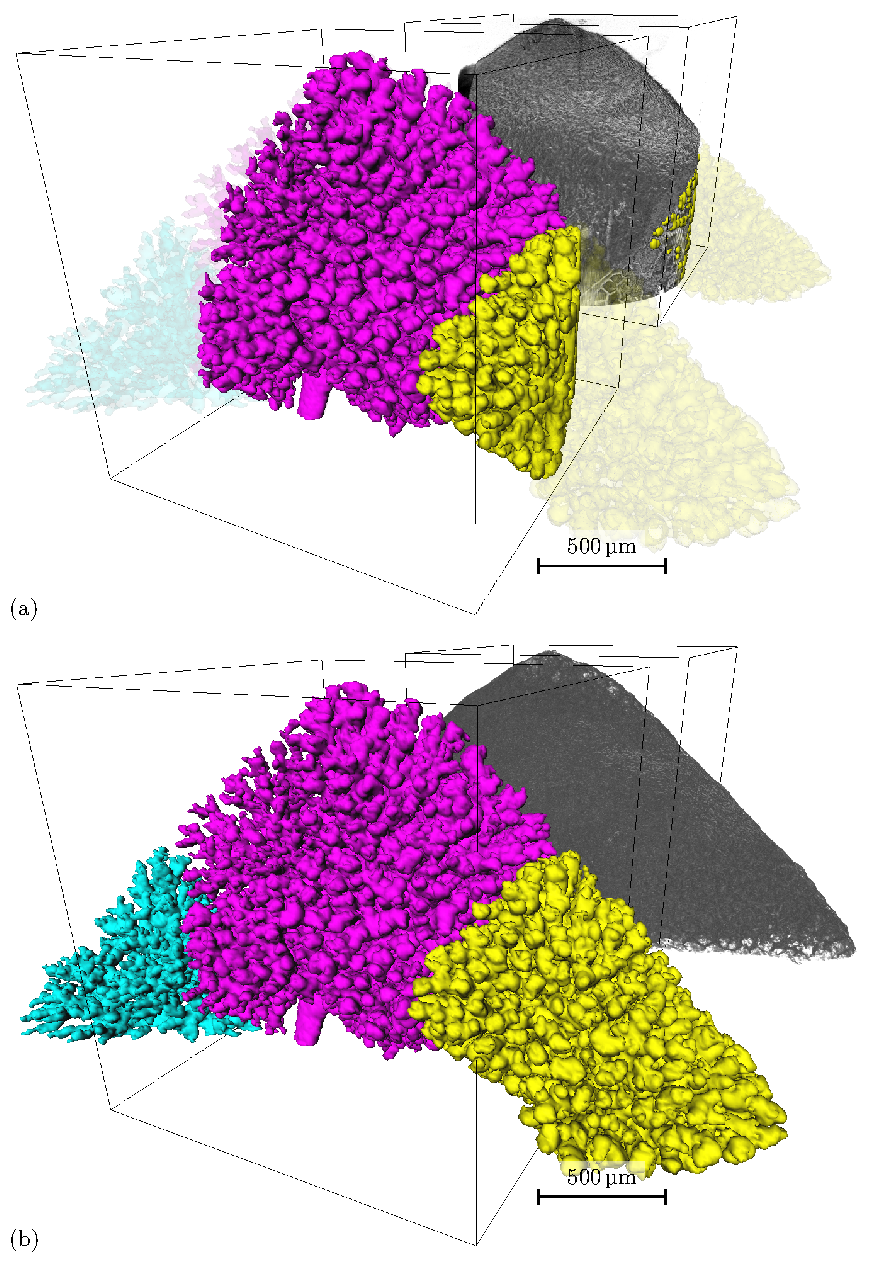
\includegraphics[width=.7\linewidth]{img/Haberthuer2010/Fig05-ConvVsWfs}
	\label{fig:s2-wfs}
\end{figure}

\subsection{Performance of the scanned protocols}
The performance of the 19 protocols has been quantified using the difference image between binarized slices of the gold standard protocol and each protocol to be assessed. The slices have been thresholded according to \citet{Otsu1979}. The difference value ($E_{norm}$) plotted in Figure~\ref{fig:NormalizedErrorPlot} was calculated for each protocol $i=$1--19 (B--T) according to equations~\ref{eq:errorcalculation-a}--\ref{eq:errorcalculation-c}. Using a thresholded slice $k$ of each protocol $i$ ($Slice_{i_{k}}$) and the corresponding slice $k$ of the gold standard protocol $B$ ($Slice_{B_{k}}$) the absolute difference image ($D_{i_{k}}$) of these two slices $k$ was calculated. The sum of all pixels of this difference image yields a value ($E_{i_{norm_{k}}}$) for the difference of the examined slice $k$ of protocol $i$ with the corresponding slice of the gold standard protocol B.
\begin{eqnarray}
	D_{i_{k}} &=& |Slice_{B_{k}}-Slice_{i_{k}}|\label{eq:errorcalculation-a}\\%
	E_{i_{norm_{k}}} &=& \sum_{x}\sum_{y} D_{i_{k}}\label{eq:errorcalculation-b}\\%
	E_{i_{norm}} &=& \overline{E_{i_{norm_{k}}}}\label{eq:errorcalculation-c}%
\end{eqnarray}

This combined difference value ($E_{i_{norm_{k}}}$) was calculated for 205 regularly spaced slices (%
%$i=1:5:1024$%
every fifth slice) of the full dataset. The mean ($\overline{E_{i_{norm_{k}}}}$) difference value for all slices was normalized to the scanned quality-steps from 16--\SI{116}{\percent} (as stated in Table~\ref{tab:protocols}) and plotted with its standard deviation ($\sigma(E_{i_{norm_{k}}})$). For the purpose of comparison, data has been normalized.

As expected, the calculated quality of the reconstructions representing the different protocols decreases as a function of total number of obtained projections (Figure~\ref{fig:NormalizedErrorPlot}). The calculated error of the different protocols (normalized difference value, blue diamonds) shows the experimental results obtained from actual scans of lung tissue. The plots for the simulation as defined in section~\ref{sec:quality guided protocols} (red dots) and the normalized difference value are not perfectly in agreement, but show the same trend. The linear regression for the simulation shows a steeper decrease for the quality ($y_{Sim}=0.6936x+26.891$) than the linear interpolation for the experimental data ($y_{Exp}=0.5833x+20.226$). The linear regression coefficient for both the linear interpolations are comparable ($R^{2}_{Sim}=0.8287$, $R^{2}_{Exp}=0.7868$).

\begin{figure}
	\centering
	\caption{Plot of normalized difference Value ($E_{i_{norm}}$, blue diamonds) for the 19 scanned protocols overlaid over Quality-plot (red dots) obtained from the simulation (described in section~\ref{sec:quality guided protocols}. The normalized Error has been calculated using the difference image of each protocol $i$ with protocol B. The error bars for each protocol show the standard deviation of the error calculated for 205 of the 1024 slices. Note that the scale of the error was normalized to 20--\SI{100}{\percent}, so that both the quality from the simulation and the error are directly comparable. The abscissa shows the scanning time in percentage of time used for the gold standard scan. Protocol T on the far left corresponds to the fastest scanning time, protocol B on the far right to the slowest. The protocols in between are shown from T--B for increasing percentage of the scanning time.}
	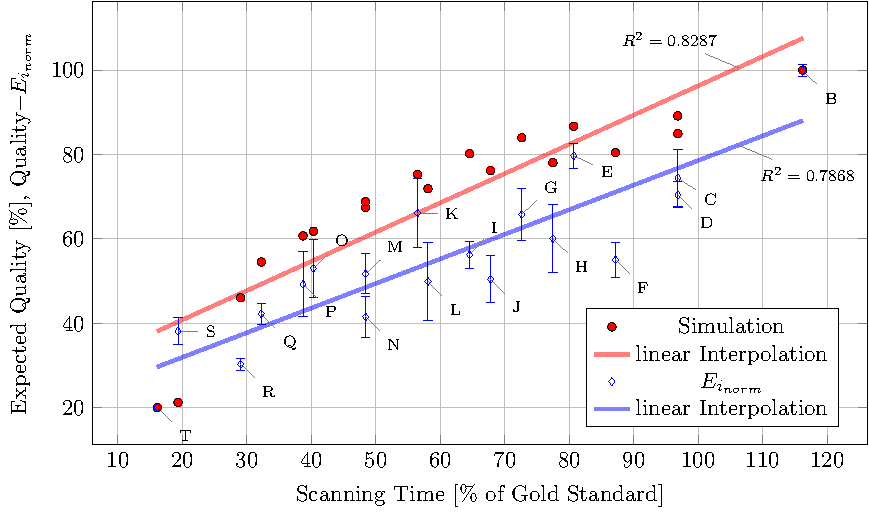
\includegraphics[width=\linewidth]{img/Haberthuer2010/Fig06-Plot}
	\label{fig:NormalizedErrorPlot}
\end{figure}

\subsection{Three-dimensional visualization of different protocols}
\label{subsec:comparison}
The tomograms of the different protocols were three-dimensionally analyzed and visualized using MeVisLab (Version 2.0 (2009-06-09 Release), MeVis Medical Solutions AG and Fraunhofer MEVIS - Institute for Medical Image Computing, Bremen, Germany). Airway segments were extracted using a threshold interval based region growing algorithm~\cite{Zucker1976}. A seed point for the region growing algorithm was manually defined in the most proximal slice for each independent airway segment. The coordinates of the seed points were kept constant for protocol B--T, allowing direct comparison between the airway segment reconstructions of the different protocols. Airway segments extracted for protocol B, L and T are shown in Figure~\ref{fig:BvsT}.

Protocol B corresponds to a slightly oversampled gold standard scan, obtained with total 15732 projections, recorded in \SI{66}{\minute}. Protocol L was obtained in \SI{35}{\minute} with total 7866 projections. Protocol T was obtained in \SI{12}{\minute} with 2185 projections for all three subscans. The tomographic dataset from protocol B was reconstructed from 5244 merged projections, the dataset from protocol L was reconstructed from 2622 merged projections and the dataset from protocol T was reconstructed using only 874 merged projections. Even though protocols L and T were scanned while violating the sampling theorem and with a total scanning time reduction of \SI{40}{\percent} (L) or more than \SI{86}{\percent} (T), the samples still appear to be identical to the gold standard protocol in the low-resolution three-dimensional visualizations shown in Figure~\ref{fig:BvsT}(a)--(c).

Figure~\ref{fig:BvsT}(d)--(f) show isosurface visualizations of the border between airspace and lung tissue as cubic regions of interest (256 pixels wide, location inside the sample is marked as blue cube in Figure~\ref{fig:BvsT}(a)--(c)). Because of experimental constraints, the cutline between the individual subscans could not be defined with a precision of one single pixel. As a consequence, the clipping plane does not lie in exactly the same position. This explains the appearing and disappearing holes in Figure~\ref{fig:BvsT}(d)--(f).

Even with the higher magnification, the reconstruction of protocol L in Figure~\ref{fig:BvsT}(e) appears nearly identical to the reconstruction of the region of interest of protocol B (fig.~\ref{fig:BvsT}(d)). The isosurface of the region of interest of protocol T shown in Figure~\ref{fig:BvsT}(f) appears rougher than the isosurface of protocol B. This roughness is introduced through ray-like artifacts visible in the original slice of the dataset of protocol T (not shown). These artifacts are the consequence of a strong subsampling. With the acquisition of only 874 projections instead of the required 5139, the sampling theorem is far from being satisfied. However, even with this strong undersampling, segmentation, three-dimensional reconstruction and visualization of the sample is still possible.

%\onecolumn
\begin{figure}
	\centering
	\caption{Comparison of three-dimensional visualizations. %
			(a)--(c): Three independent airway segments (cyan, magenta, yellow) of tomographic datasets obtained with protocol B, L and T, extracted using a region growing algorithm. A cubic region of interest (blue) with a side length of 256 pixels (corresponding to \SI{379}{\micro\meter}) is marked inside the leftmost segment for all protocols. %
			(d)--(f): Detailed view of isosurfaces of the lung tissue inside the blue ROIs for protocol B, L and T, respectively. Note the increasing surface roughness in the alveolar surfaces for subfigures (e) and (f).}%
	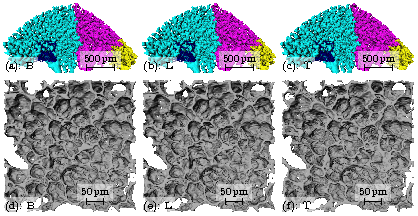
\includegraphics[width=\linewidth]{img/Haberthuer2010/Fig07-B-L-T}
	\label{fig:BvsT}
\end{figure}%
%\twocolumn%

For further analysis four regions of interest with a side length of 256 pixels have been extracted for each of the protocols B, L and T. The three-dimensional location of these ROIs inside the sample is shown in Figure~\ref{fig:roi3d}.

\begin{figure}
	\centering
	\caption{Overview of the location of the four regions of interest where the histogram of the euclidean distance transformation distribution has been calculated. Grey: Semitransparent volume rendering of the lung tissue sample. Red: Four regions of interest, extracted to calculate the distance transformation. The labels of the ROIs conform to the legends in Figure~\ref{fig:DTFplots}.}%
	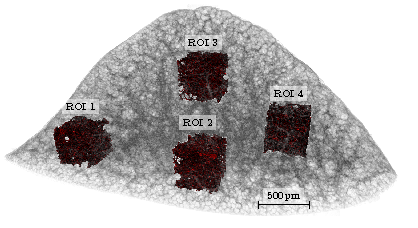
\includegraphics[width=\linewidth]{img/Haberthuer2010/Fig08-ROIs}
	\label{fig:roi3d}
\end{figure}

Each of the ROIs has been binarized using an algorithmically determined threshold~\cite{Otsu1979} and small particles inside the segmented airspace lumen have been removed using a connected component analysis. Subsequently, the euclidean distance transformation~\cite{Danielsson1980} has been calculated for each thresholded ROI.

For comparison, the histogram of the euclidean distance transformation has been plotted for all four regions of interest in each protocol (B, L and T).

\begin{figure}
	\centering
	\caption{Histogram-Plots for each of the of four ROIs, each showing the histogram of the distance transformation for the protocols B, L and T.}%
	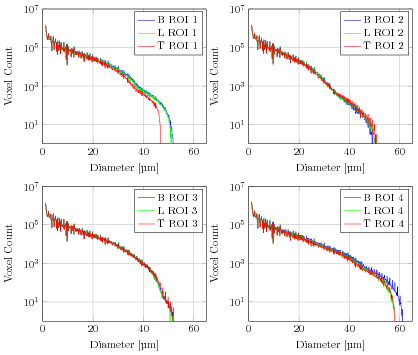
\includegraphics[width=\linewidth]{img/Haberthuer2010/Fig09-DTF}
	\label{fig:DTFplots}
\end{figure}

Figure~\ref{fig:DTFplots} shows logarithmic plots of the histogram distributions for the four selected ROIs; the blue, green and red plot show the histograms of the distance transformation of Protocol B, L and T, respectively. For all four regions of interest, the distribution of the euclidean distance transformation is very similar, only for larger airway diameters (between 50--\SI{60}{\micro\meter}) we see a detectable difference in the regions of interest 1 and 4, located in the lateral parts of the sample. If we remember that the histogram is plotted with a logarithmic y-axis, we see that the difference of the histograms is only visible for several hundred voxels.

Even when reducing the sample acquisition time by \SI{84}{\percent} of the gold standard scan (T vs. B), the distance transformation histograms of the shown regions of interest are very similar and therefore no relevant structural differences are introduced.

As a further proof of concept we scanned and reconstructed a rat lung sample with five scanning positions, resulting in a nearly five-fold (4.74$\times$) increase in field of view from slices with a size of 1024$\times$1024 pixels to a size of 4852$\times$4852 pixels (1.52$\times$\SI{1.52}{\milli\meter} to 7.18$\times$\SI{7.18}{\milli\meter}) at a voxel side length of \SI{1.48}{\micro\meter}. A three-dimensional visualization of the boundary between airspace and tissue in this reconstructed dataset validated the wide field scanning method for further increases in the available field of view (data not shown).

\section{Discussion}\label{sec:Discussion}
We present a method to laterally increase the field of view of tomographic imaging systems operated in parallel beam geometry and would like to call this method wide field synchrotron radiation based x-ray tomographic microscopy (WF-SRXTM). We defined scanning protocols for the optimization of the total imaging time versus the expected imaging quality, enabling a very fast acquisition of lower quality tomographic datasets, or acquisition of very high quality datasets in a longer time.

Even if the reduction in scanning time does introduce minor artifacts in the three-dimensional reconstruction, as shown in Figure~\ref{fig:BvsT}, an automated segmentation of the relevant features in the sample is still possible, even for protocols with greatly reduced scanning time. 

Additionally, shortening the scanning time also reduces the radiation damage even though, for this study, this was not an issue. Obviously, a reduction of the imparted dose to the sample is crucial when radiation sensitive sample are investigated. With a
suitable protocol the dose can be reduced by \SI{84}{\percent} (Table~\ref{tab:protocols}), which might be a significant step towards tomographic imaging of sensitive samples using ultra high resolution and enhanced field of view. 

The field of view was increased three-fold by merging projections from three partially overlapping scans and reconstructing these resulting projections using the standard workflow at the TOMCAT beamline (Figure~\ref{fig:wide-field-scan-results}). As a consequence of the sampling theorem, an increased amount of projections had to be acquired, thus increasing the acquisition time. To overcome this limitation, we defined multiple scanning protocols with a reduced amount of total projections and thus reduced acquisition time and delivered dose (Table~\ref{tab:protocols}). All of these protocols were evaluated for the quality of the resulting reconstructions and compared to a gold standard scan. We have shown that the resulting quality can be simulated prior to scanning and thus provide a tool to choose a suited scanning protocol, based on the demands for scanning time optimization and quality of the resulting tomographic dataset (Figure~\ref{fig:NormalizedErrorPlot}). 

Reducing the amount of projections for the central of the three subscans may be performed with a minor loss of fidelity in the resulting reconstructions. Let us compare protocols D/E and H/I. For protocols E and I we acquired half the amount of projections for the central subscan $\textrm{s}_{2}$ as compared to protocols D and H. In both cases we reduce the scanning time by \SI{17}{\percent}, but keep the quality of the scan on a comparable level (D: $\SI{70}{\percent}\pm3.09$ vs. E: $\SI{80}{\percent}\pm3.01$, H: $\SI{60}{\percent}\pm8.08$ vs. I: $\SI{56}{\percent}\pm3.23$).
% B--C = 13110/15732 = 0.8333, 100%--89%
% D--E = 10925/13110 = 0.8333, 85%--87%
% H--I = 8740/10488 = 0.8303; 78%--80%
We show that the interpolation of missing projections does not introduce relevant errors in the resulting tomographic datasets.

For protocols with an equal amount of total projections, but differing amount of projections for the individual subscans (C/D and M/N) we observed minor differences in reconstruction quality. The qualities $E_{i_{norm}}$ of protocols C and D lie within their respective standard deviation ($\SI{74}{\percent}\pm6.81$ vs. $\SI{70}{\percent}\pm3.09$), and the qualities of protocols M and N are comparable ($\SI{52}{\percent}\pm4.71$ vs. $\SI{42}{\percent}\pm4.78$). Both protocols C and M are scanned without oversampling the central subscan, making interpolation necessary, for protocols D and N we simply stitched the projections of the three subscans. Note that for protocol N we do undersample the outer parts of the sample. When deciding between two protocols with the same amount of total projections, it is thus desirable to favor the protocol where the central scan is not oversampled (i.\,e. choosing protocol C instead of D). Even if this introduces additional computing time to interpolate projections prior to reconstruction, these protocols show an increased quality compared to protocols where the central scan is oversampled. Since an oversampling of the central scan does not add much to the total reconstruction quality and the outer parts of the sample contribute more to the total area of the projections, choosing a protocol where the sampling theorem is satisfied better for those parts of the sample is favorable (i.\,e. favouring protocol M to protocol N).

With the defined protocols we open the possibility for the end-user to choose an acquisition mode suited to fulfill the constraints on number of samples to be scanned within the allocated beamtime and desired quality of the reconstructed datasets.

Additionally, two special use-cases for different protocols are worth mentioning. First, if the user needs a very quick overview over samples at high resolution, a time-saving protocol can be used. This is especially the case, if the integrity of the sample can only be judged with a tomographic scan. Based on the quick scan the right samples for high resolution scans may be selected. It has to be mentioned that a quick overview could---in principle---be obtained with a low-resolution scan, which usually automatically accommodates a larger field of view. However, the resolution of such an overview scan is not always sufficient to detect interesting features in the samples which might be damaged.

We have shown that the field of view of parallel beam tomographic end-stations can be increased up to five-fold and have routinely reconstructed multiple tomograms with a three-fold increase in field of view. The shown acquisition protocols are theoretically expandable for more than five subscans, although the reconstruction of wide field scans with seven or more subscans would require an extremely powerful data processing infrastructure. The datasets shown in Figure~\ref{fig:BvsT} are binned scans resulting in datasets of 1024 slices, each with a size of 2792$\times$2792 pixels at \SI{8}{\bit} gray value depth, which adds up to a total size of the dataset of approximately \SI{7.5}{\giga\byte}. If we assume an unbinned scan with seven overlapping subscans, the size of one stitched projection will be approximately 14000$\times$14000 pixels. The full dataset will consist of 2048 such slices, which would add up to a total size for the full dataset of approximately \SI{383}{\giga\byte}.

Even if the amount of data to handle is huge, a wide field scan with a five-fold increase in field of view remains interesting, since it would enable the end-user to selectively reconstruct only regions of interest from large samples with ultra-high resolution. Up to now, a two-step process was required to scan precisely defined regions from samples larger than the field of view. This process involved the use of different magnifications, two separate beamtimes and a precise registration of the samples between those beamtimes.

\section{Summary}\label{summary}
A method to increase the lateral field of view of tomographic imaging has been established, which enables the high-resolution tomographic imaging of large samples that are wider than the field of view of the optical setup in multiple semi-automatically combined steps. Tomographic datasets of entire rat lung acini have been acquired with an enhanced field of view using WF-SRXTM.

Different optimized scanning protocols for covering a large field of view have been validated and are now provided for the end-users of the TOMCAT beamline. End-users now have the possibility to choose suitable scanning protocols depending on a balance between acquisition time and expected reconstruction quality. Depending on this balance, a reduction of the image acquisition time by \SI{84}{\percent} is possible, while keeping the quality of the reconstructed tomographic dataset on a level still permitting automated segmentation of the lung structure and surrounding airspace, as shown in section~\ref{subsec:comparison}. The reduction in acquisition time obviously reduces the time during which the sample is irradiated by synchrotron radiation and thus reduces the radiation dose inflicted on the sample.

\section{Acknowledgments}
This work has been funded by the grants 3100A0-109874 and 310030-125397 of the Swiss National Science Foundation. We thank Mohammed Ouanella for his excellent technical assistance and Volker Dicken from Fraunhofer MEVIS for the fruitful discussion concerning the euclidean distance transformation. Dan Ward kindly checked the English of the manuscript.